\chapter{Grundlegende Begriffe}
\label{ch:basics}
In folgendem Kapitel werden die Grundlagen erläutert, welche für spätere Kapitel benötigt werden. 
Es wird kurz auf die Historie von Turing Tests eingegangen, 
bevor die verschiedenen CAPTCHA-Methoden und Alternativen grundlegend erläutert werden. 
Zuletzt wird ein grundlegendes Verständnis für UX geschaffen.

\section{Turing Tests}
\label{ch:basics:turing}
Alan M. Turing $($1912-1954$)$ ist einer der Mitbegründer der heutigen Informatik 
und legte mit seiner Forschung einen der Grundsteine für die Entwicklung von künstlicher Intelligenz. 
In seinem Paper ''On computable numbers, with an application to the Entscheidungsproblem'' \cite{turing} 
beschreibt er den Umgang mit ''computable numbers'' und wie diese durch eine - später als Turing Machine bezeichnete - Maschine berechnet werden könnte.
Diese Turing Machine ''[\dots] ist damit ein Model physischer digitaler Computer, die zu jener Zeit jedoch noch nicht existieren. [\dots]'' \cite[p.4]{pallay2020turing}
Hierbei kam er zur Erkenntnis, dass sich nicht alle mathematischen Probleme durch eine fixe Vorgehensweise, also einen Algorithmus, lösen lassen. 
Erst später wurde festgestellt, dass Turing Maschinen und Computer jeweils vom anderen simuliert werden können. \cite[p.647]{geniusofturing} \cite[p.4]{pallay2020turing} %TODO: Formulierung

Turing beschäftigte sich bis zu seinem frühen Tod weiterhin mit maschineller Intelligenz 
und ''[\dots] beschreibt [\dots] das, was man heute als [\dots] künstliche Intelligenz bezeichnet.'' \cite[p.10]{pallay2020turing}
Durch seine Überzeugung, dass eines Tages maschinelle Intelligenzen entwickelt werden (können), 
entwickelte Turing in seinem Paper ''Computing Machinery and Intelligence'' \cite[p.23ff]{turing2009computing} 
eine Methode des Testens der Intelligenz einer Maschine. 
Um die Notwendigkeit von genauen Definitionen zu vermeiden, nutzt er deshalb ein Abwandlung eines Verfahren - des ''imitation games''. 
''Hierbei kommuniziert ein Juror maschinen-schriftlich mit einem Menschen und einer Maschine.'' \cite[p.12]{pallay2020turing}
Sollte der Juror nicht feststellen können, welcher Gesprächspartner der Mensch ist, gilt der Test als bestanden. \cite[p.11ff]{pallay2020turing}

Dieses Verfahren wird heute oftmals als Turing Test bezeichnet. 

\section{CAPTCHA}
%label
Bei der Abkürzung CAPTCHA handelt es sich um ''completely automated public turing tests to tell computers and humans apart''. 
Sie werden genutzt, um Webseiten vor Angriffen durch Bots zu schützen. 
Dies wird durch die im vorherigen Kapitel bereits erläuterten Turing Tests erreicht. 
Hier ist das Ziel, durch für Computer schwer, für Menschen jedoch leicht zu verarbeitende Medien, das Tracken von Mausbewegungen
oder das Prüfen der Browseraktivität zu prüfen, ob es sich wirklich um eine*n menschliche*n Nutzer*in handelt.

Fast identisch zu CAPTCHA sind sogenannte HIP – ''Human Interactive Proofs''. 
Dieser Begriff hat sich entwickelt, da manche Tests nicht ''public'' sind. \cite[p.1]{chellapilla} \cite{tutorial} 

\subsection{Arten von CAPTCHA}
Nachfolgend werden verschiedene Arten von CAPTCHAs grundlegend erläutert.
Textbasierte CAPTCHA waren bereits 2008 die am häufigsten verwendete Art von CAPTCHA.
Sie zeichnen sich durch eine Verzerrung eines Wortes oder mehreren Wörtern aus, sodass diese für Bilderkennungstools nicht erkennbar sind.
Eine weitere Variante textbasierter CAPTCHA ist die einer einfachen Rechenaufgabe. 
Auch hier soll erreicht werden, dass ein Bot die angegebenen Zahlen nicht korrekt erkennen kann und die Gleichung somit nicht lösen kann. \cite{usabilityofcaptchas} \cite[p.75]{surveyofresearch} \cite{shinde2018DIFFERENTTO} %TODO SEITEN!!!!!!!!!
Bei der Darstellung dieser Zeichen und Symbole können verschiedene Ansätze verfolgt werden.
\citeauthor{surveyofresearch} beschreiben hierbei ``anti-segmentation techniques'' und ``anti-recognition techniques''. \cite[p.76]{surveyofresearch}
Anti-Segmentation Techniques zielen darauf ab, das Separieren der einzelnen Buchstaben durch Algorithmen zu erschweren. 
Um dies zu erreichen, gibt es verschiedene Herangehensweise.
Eine von diesen ist 

Hollow: A main feature of hollow CAPTCHAs is to use
contour lines to form connected characters with the aim of
improving security and usability simultaneously, as the
connected characters are hard to segment, but are easily seen
by humans. Unfortunately, this mechanism is not as secure as
people expected, research by Gao [17] used a generic method
to combine segmentation with recognition to break a series of
really hollow CAPTCHAs with success rates ranging from
36% to 89%.

CCT and overlapping: crowing characters together
(CCT) and overlapping try to make segmentation more
difficult by squeezing characters together. However, it may
reduce user friendliness. For instance, reference [13] broke the
Google CAPTCHA and reCAPTCHA [14] with success rates
of 46.75% and 33%, respectively. A novel method was also
presented in [15] to attack CCT-based CAPTCHAs, achieving
success rates from 27.1% to 53.2%.

Noise background: The noise background mechanism
hides the position of the characters. Regrettably, Google’s
reCAPTCHA, which uses Street View images, is broken by a
method imitating the probability of a sequence proposed in
[21]. In addition, Gao [19] used some image processing
techniques iteratively to break PayPal’s CAPTCHA.

Two-layer structure: A two-layer structure is a vertical
combination of two single-layers CAPTCHA. The most
critical issue in breaking this mechanism is segmentation,
which cannot be solved by common segmentation methods.
Gao [18] presented a novel two-dimensional segmentation
approach to separate a CAPTCHA image along both vertical
and horizontal directions and achieved a success rate of
44.6%.
76

Multifonts, Rotation, Waving: These three methods are
designed to increase the diversity of each character, thereby
increasing the number of features needed to identify each class
by machine.

Large character set: A large character set makes the
solution space much larger than that of traditional text
CAPTCHAs. It usually chose Chinese, Japanese, etc. 
\cite{surveyofresearch}

\begin{figure}
    \centering
    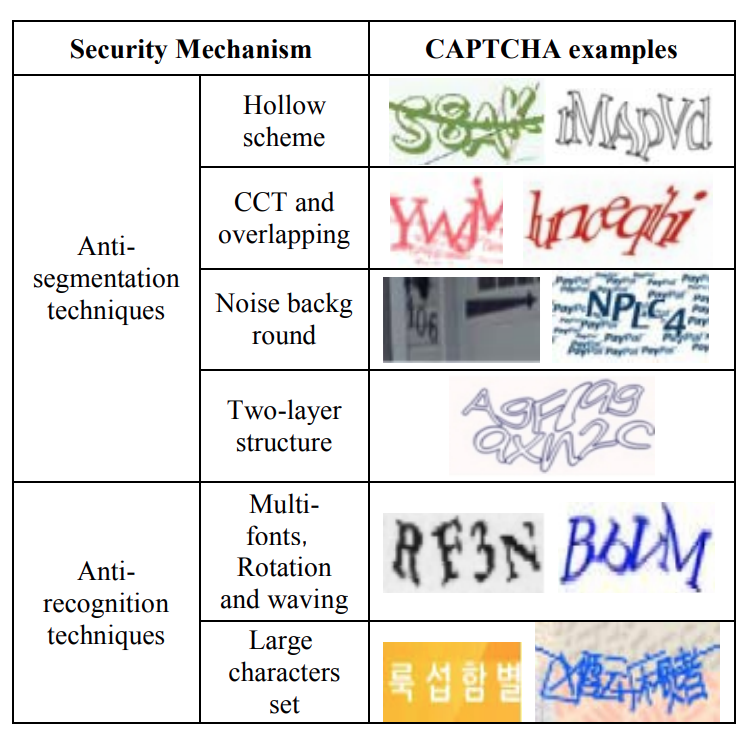
\includegraphics{gfx/mygraphics/unbedingtaustauschen1.png}
    \caption{textbasierte Beispiele die ich unbedingt noch austauschen muss, weil sie aus \cite{surveyofresearch} sind}
    \label{fig:pr0grammcaptcha}
\end{figure}

Es gibt verschiedene Arten von bildbasierten CAPTCHAs. 
Die wohl bekannteste ist ein in Quadrate aufgeteiltes Bild, wobei man jene Quadrate auswählen soll, welche einen bestimmten Gegenstand enthalten.
Eine Variation dieses CAPTCHAs besteht aus einer Zahl verschiedener Bilder, von denen eine Teilmenge ebenfalls ein gesuchtes Objekt beinhalten.
%Discord CAPTCHA: PFERDE AUS WOLKEN!!!!!

%Audiobasiert

%Logik

% Gamification

\begin{figure}
    \centering
    \subfloat[\centering]{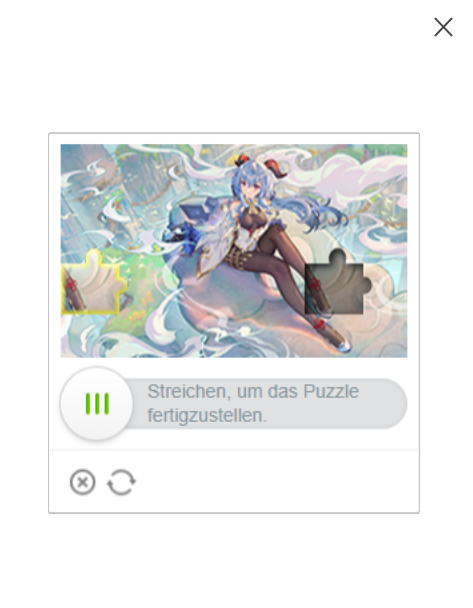
\includegraphics[width=5cm]{gfx/mygraphics/genshincaptcha.png}}
    \qquad
    \subfloat[\centering]{
\includegraphics[width=5cm]{gfx/mygraphics/hoyoversecaptcha.png}}
    \caption{Gamification-CAPTCHA bei Login in Genshin Impact $(a$) und dem Forum Hoyolab $(b$)}   
\end{figure}

Eine aktuell viel genutzte Form der Spam-Prävention ist reCAPTCHA v3 von Google. 
Hier werden keine Turing Tests durchgeführt. 
Vielmehr wird anhand verschiedener Faktoren bewertet, ob es sich um einen Bot oder einen Menschen handelt.
Was genau diese Faktoren sind, gibt Google aus Sicherheitsgründen nicht Preis. 
Denkbar ist jedoch die Betrachtung von Cookies oder der Häufigkeit von Anfragen durch die gegebene IP-Adresse.
In der Dokumentation wird angegeben, dass ein Score von 0.0 bis 1.0 vergeben werden kann. 
Hier gilt: Je niedriger der Score, desto wahrscheinlicher handelt es sich um einen Bot statt eines ``echten'' Nutzers. (Vgl. \cite{recaptchadoc})
Laut Google selbst soll reCAPTCHA v3 eine sehr gute Nutzererfahrung bieten, da es kaum bis gar keine Zuarbeit durch den Nutzer verlangt. \cite{googleblog:recaptcha}
ReCAPTCHA kann durch das Fehlen eines klassischen Turing Tests auch als eine CAPTCHA-Alternative interpretiert werden.

\begin{figure}
    \centering
    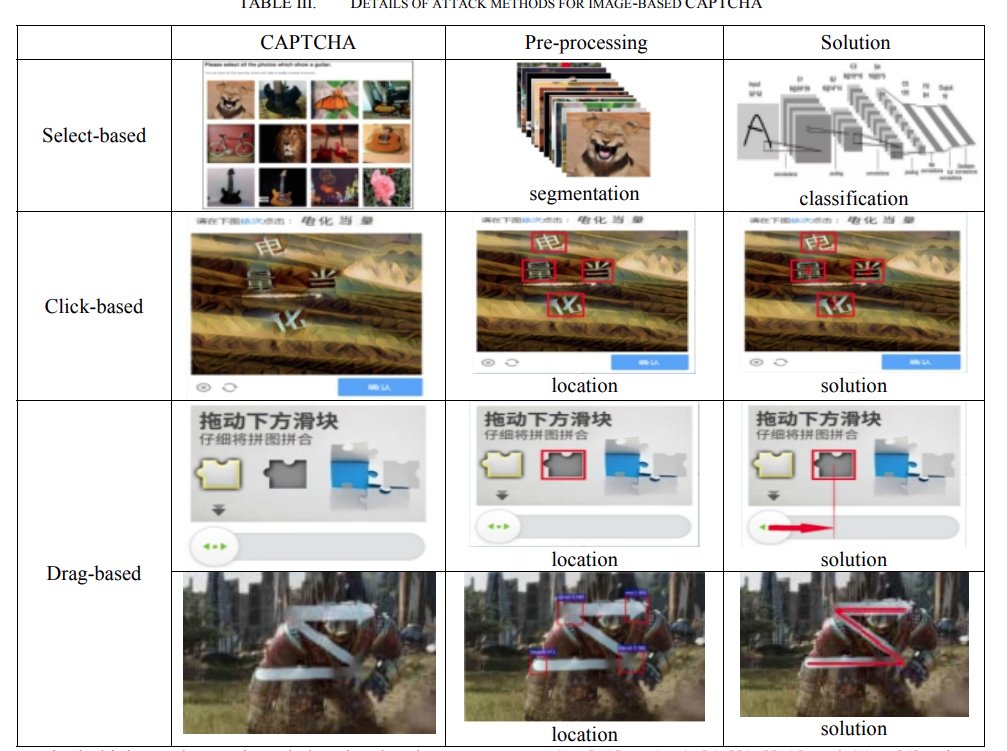
\includegraphics{gfx/mygraphics/unbedingtaustauschen2.png}
    \caption{bildbasierte Beispiele die ich unbedingt noch austauschen muss, weil sie aus \cite{surveyofresearch} sind}
    \label{fig:pr0grammcaptcha}
\end{figure}

\subsection{Alternativen zu klassischen CAPTCHA}
%anti spam plugins
%multi faktor authentifikation
%biometrie
Eine weitere Alternative zu klassischen CAPTCHA sind sogenannte Honeypots. 
Geprägt wurde der Begriff erstmals im Kalten Krieg als Spionagetechnik eingesetzt wurde. \cite[p.2]{joshi:2011} 

Auch heute werden Honeypots eingesetzt, und zwar in der IT-Sicherheit. 
Oft werden sie mit ``Fallen'' assoziiert, welche Hacker anlocken sollen. 
Dadurch können Angriffsarten analysiert werden und ''echte'' Systeme werden nicht angegriffen.

Doch auch im Kontext der Unterscheidung von Menschen und Maschine gibt es Honeypots. 
So kann man HTML-Inputfelder durch CSS verstecken, sodass diese nur durch Bots, welche den Quellcode der Seite scannen, ausgefüllt werden 
und nicht durch Menschen, da diese das Textfeld nicht sehen. 
Bei der Prüfung der Inputs kann nun überprüft werden, ob ein Bot in die Falle getappt ist. 
Nachzulesen sind solche Verfahren in verschiedenen Blogposts, wie \cite{perry:2019}.


\section{UX}

Die Abkürzung UX steht für \textbf{U}ser E\textbf{x}perience und beschreibt die Erfahrungen eines Users bei der Nutzung eines Systems. 
Das Ziel ist, diese Nutzererfahrung möglichst positiv zu halten. 
Im Kontext dieser Ausarbeitung wird die Definition des  ``international standard on ergonomics of human-system interaction'' $($ISO 9241-210$)$
aus dem Jahre 2010 verwendet. 
Diese definitiert UX als die Wahrnehmungen und Resonanzen einer Person, 
welche aus der $($voraussichtlichen$)$ Nutzung eines Produkts, Systems oder Services entstehen. \cite[p.1629]{berni_borgianni_2021}

Die Nutzererfahrung bei der Wahl und Nutzung von CAPTCHA ist neben der Sicherheit ein essentieller Bestandteil.
Bei der Entwicklung einer Bewertungsmatrix soll deshalb hier der Hauptfokus liegen.
Denn wenn ein CAPTCHA schwierig zu lösen ist, oder von bestimmten Personengruppen gar nicht bearbeitet werden kann, so stört dies nicht nur den Nutzungsfluss,
sondern führt gegebenenfalls auch dazu, dass Nutzer*innen die Seite verlassen, ohne ihre gewünschte Aktion zu vollenden. 

%\cite{surveyofresearch}
